\section{Monte Carlo validation procedure}
\label{chp:evtsim:valid}


Most MC generators are programs written and maintained by authors external to the ATLAS Collaboration. Moreover, the validation of official ATLAS MC generator configurations in the ATLAS simulation infrastructure and production samples for physics analyses is critically important. To accomplish this task, an automated and central MC event generator validation procedure has been developed in ATLAS. The functionality and performance of the event simulation infrastructure, as well as constant validation of the revisions and updates of the MC generators and/or the ATLAS interface packages are carefully monitored. The validation is designed to be as uniform as possible to reduce the risk of using in physics analyses MC samples affected by problems. Comparisons  of the shapes of numerous observables across different MC generators helps in identifying a variety of problems, ranging from simple mistakes in the MC generator user-defined settings to subtle-but-intentional changes in physics modelling. To ensure that the validated quantities are relevant to physical measurements, generator-independent observables defined in a theoretically-safe and unambiguous way are monitored. In some cases, technical MC generator quantities are verified (technical validation), which helps to identify MC generator internal changes. Validation includes also matrix element, particle-level and Rivet \cite{Buckley:2010ar} validation of the process being tested. The framework used is HepMCAnalysis \cite{hepmcanalysis} that contains a collection of generator-independent validation tools based on the HepMC event record \cite{Dobbs:2001ck}. It provides  broad information about final-state objects kinematics, particle content and properties ), as well as PDF information about the event. The Job Execution Monitor (JEM) \cite{Ehses:2008zz} is a Web interface used to configure and display the predefined sets of monitored and reference samples. The results of the validation tests are quickly available and presented in a flexible website (see figures \ref{sec:evtgen:fig:jemss} and \ref{sec:evtgen:fig:jem}). The agreement between the resulting pairs of histograms is quantified with several statistical tests, which include Kolmogorov-Smirnov, Pearson's $\chi^{2}$ and a bin-by-bin methods. If no outstanding issues are found, the monitored sample is marked as ``validated'' and further distributed for large-scale MC production and use in physics analyses.


\bfig[t!]
\centering
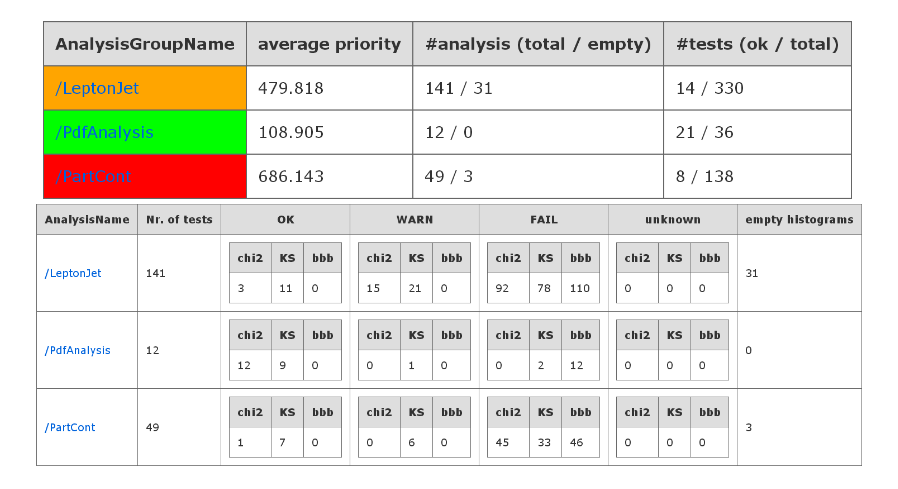
\includegraphics[width=0.8\textwidth]{figures/EvtGen/jem1.png}
\captionsetup{width=0.85\textwidth} \caption{\small A snapshot of the JEM graphical summary table with the colour-coded statistical tests output. In this example,
JEM has highlighted in red the particle content (PartCont) validation as having a large number of histograms failing the regression tests. Roughly 200 histograms produced by the HepMCAnalysis tool are validated per sample.}
\label{sec:evtgen:fig:jemss}
\efig



\bfig[h!]
\centering
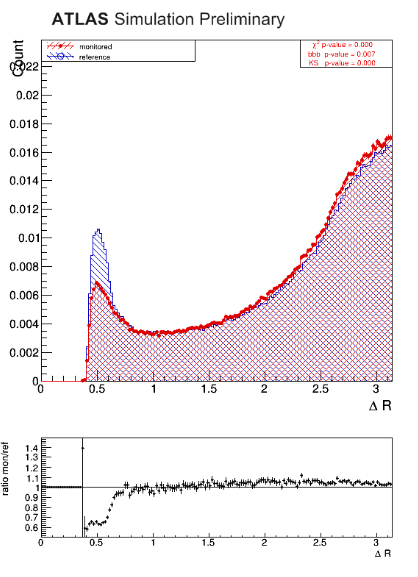
\includegraphics[width=0.5\textwidth]{figures/EvtGen/jem2.png}
\captionsetup{width=0.85\textwidth} \caption{\small Example of a distribution used for MC validation after an upgrade of the ATLAS simulation infrastruture: $\Delta R$ between the two leading $\pt$ jet in a dijet MC sample. The reference (monited) sample is displayed as a blue (red) histogram.}
\label{sec:evtgen:fig:jem}
\efig